\chapter{A model for eye information}
This chapter introduces a model for understanding and working with eye information processing systems. It is meant both as an abstract model for easily understanding the components of eye information systems and their interconnections and as a mathematical model which allows analysis of methods for information extraction and information obfuscation. The driving idea behind this approach is discovering connections between applications and being able to apply results from other adjacent scientific fields to eye information problems. Thus it is an attempt at answering the questions of how information can be quantified in a way that does not depend on specific use cases or algorithmic implementations. This leads to two things: (1) It drives the process of discovering and analysing the mechanisms by which the properties are communicated towards general concepts that provide insight into privacy in general. (2) It can, by design, lead to the creation of metrics which are usable in optimisation-based methods and thus enable data-driven method discovery.

As mentioned in the introduction, the experimental work conducted as part of this thesis is centred around iris obfuscation because it is of special interest due to the maturity of its implementation and importance in general since it is used for identification. However, the model and material is here presented for general use-cases as mentioned, due to part of the goal of the thesis being to answer what constitutes eye information and how it can be defined. This also much more clearly demonstrates the overarching purpose of the model.

The chapter is divided as follows: \todo{overview}

\section{Eye information processing systems}
\begin{figure}
	\centering
	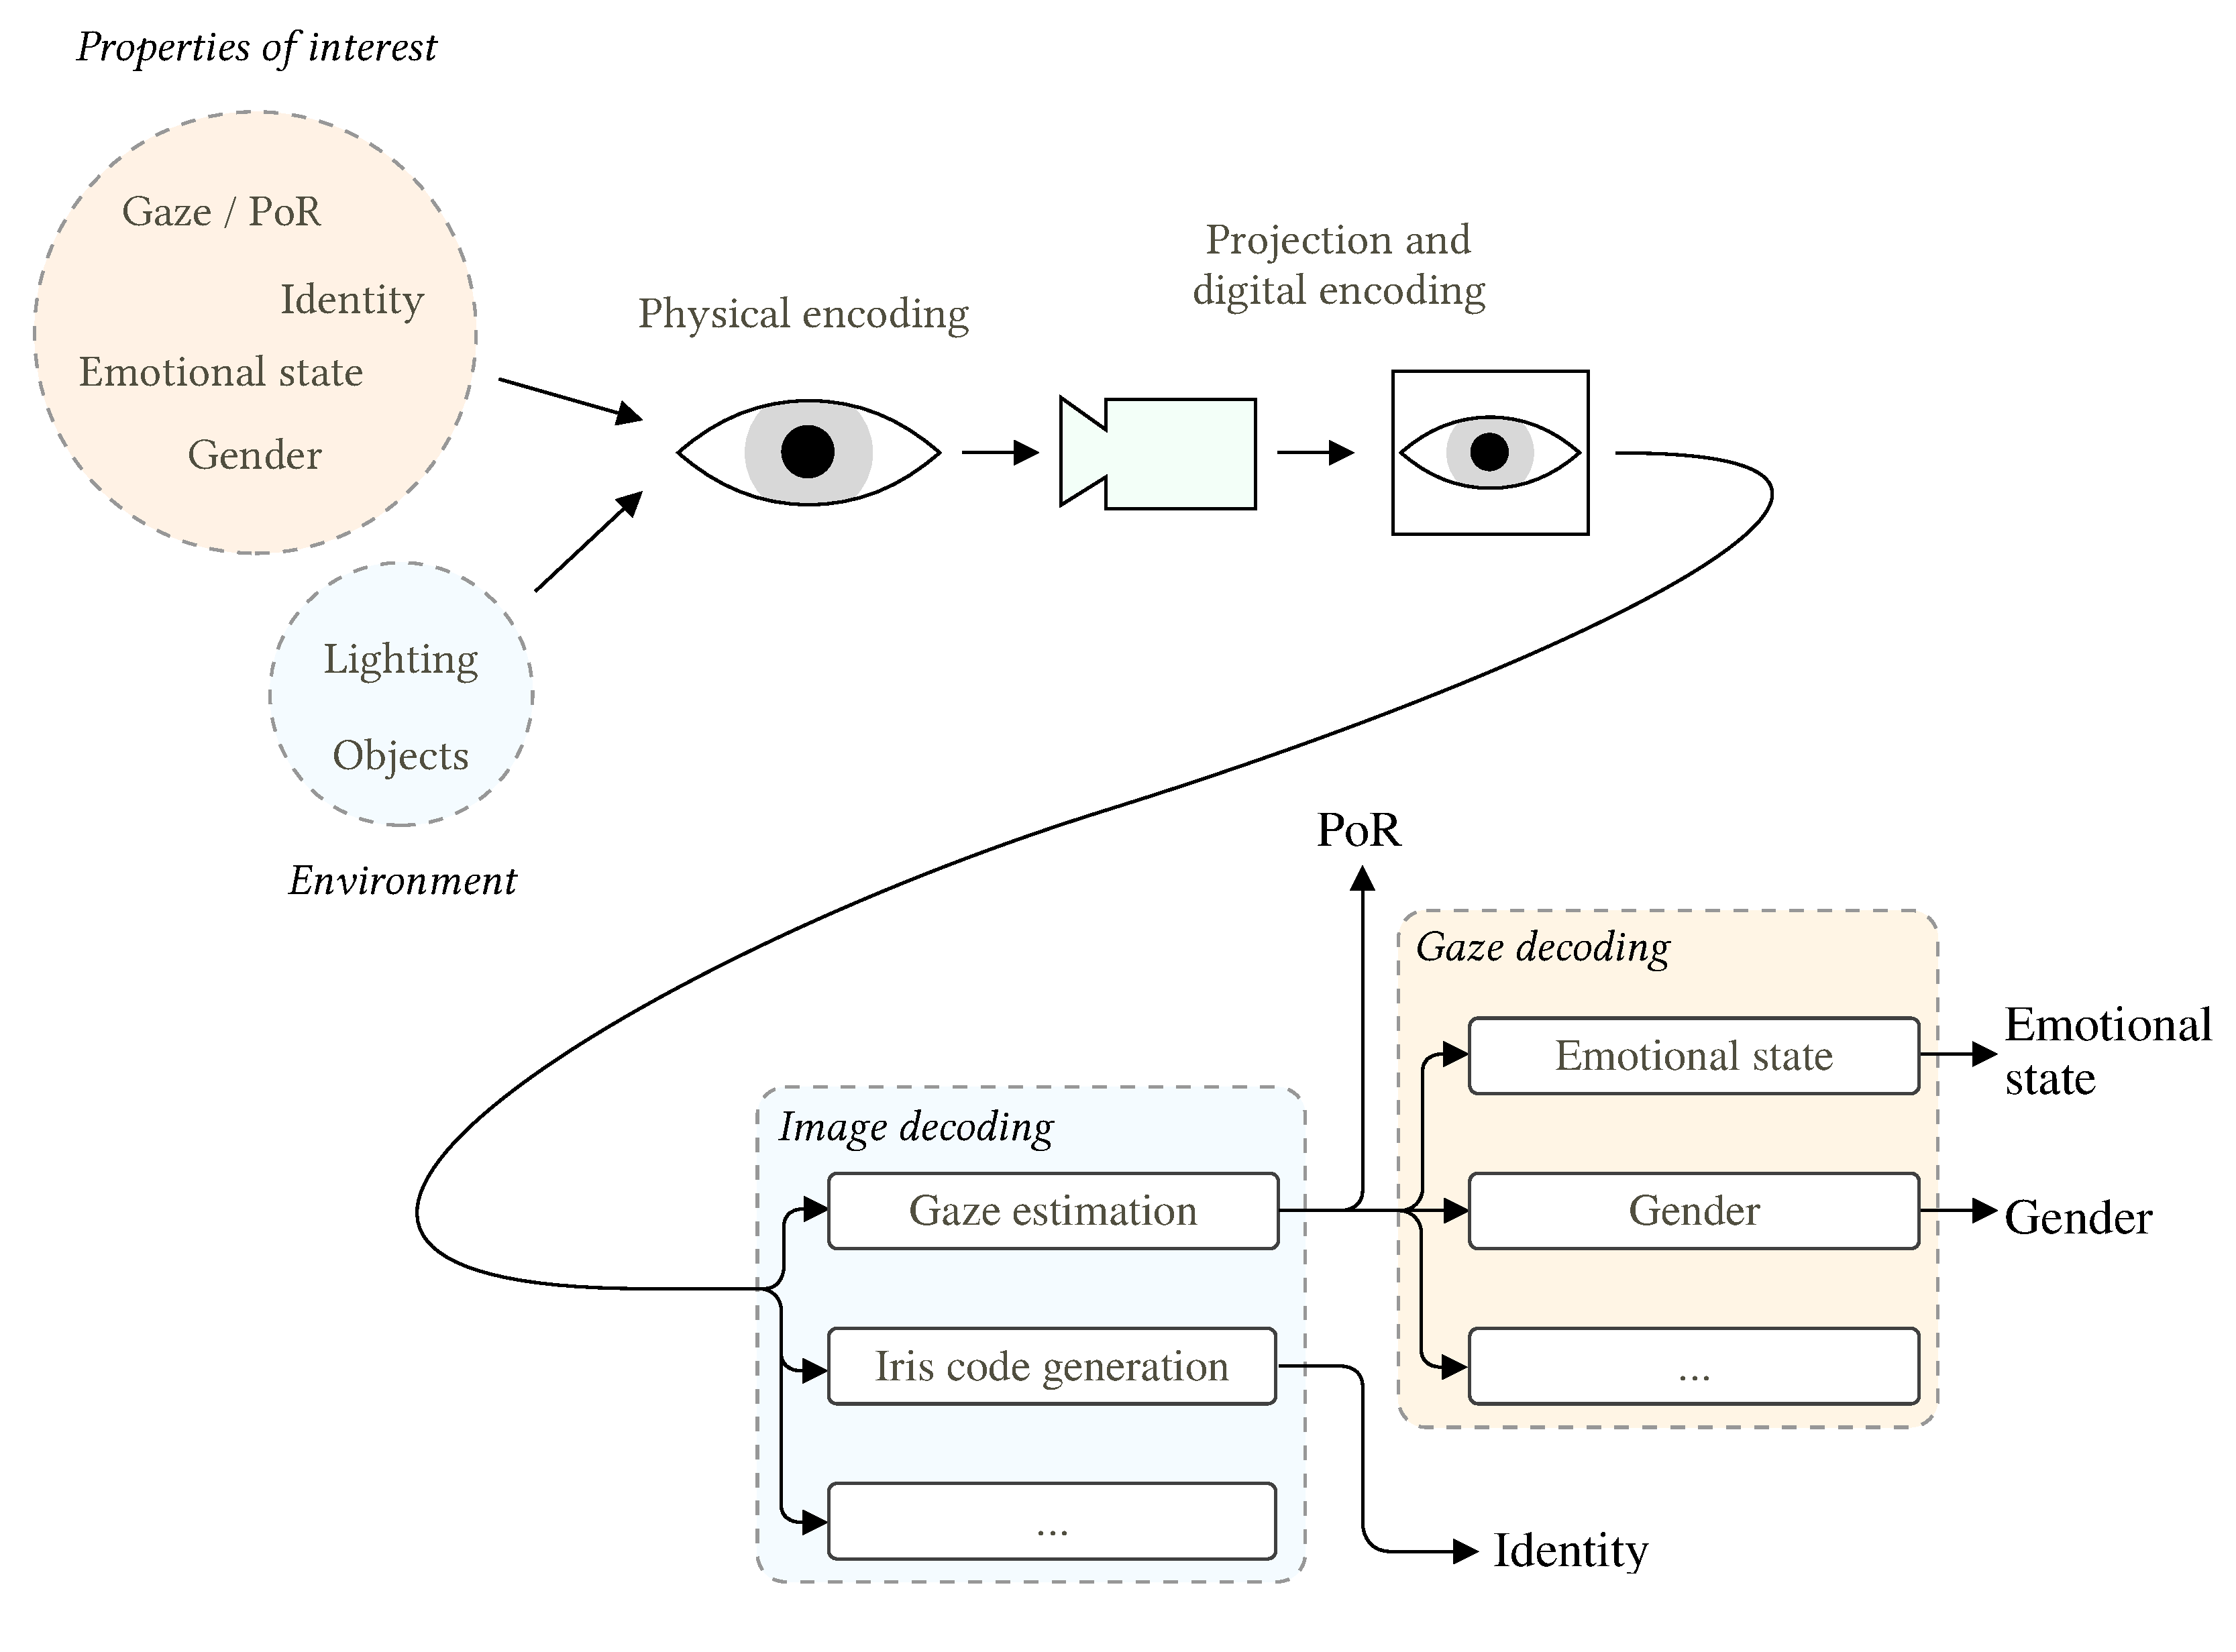
\includegraphics[width=1\textwidth]{figures/model/eye-tracking-model}
	\caption{Model overview}\label{fig:eye-tracking-model}
\end{figure}

An eye information processing system is the term used in this thesis to denote a generalisation of eye-tracking systems that includes any hardware/software system that decodes human properties using the eye as a source. \Cref{fig:eye-tracking-model} shows a simple graphical representation of the components of such a system. It includes a number of example properties, with some being decoded from the gaze signal instead of the eye images directly. This graphical representation easily contains the eye-tracking systems mentioned in (SECREF) as well as other systems such as iris-recognition. Sometimes iris-recognition may be seen as part of eye-tracking due to its typical use of eye-tracking techniques to find the iris but defining a separate term, eye information processing system, stresses the importance of the generalisability of the model.

Eye information processing systems (EIPS) closely resemble the communication model presented in (SECREF). The properties of interest affect the physical world and which thus acts as an encoding of a message, where the message is the properties. As in more typical communication systems, multiple messages, i.e. properties in EIPS, may be encoded into a single signal. Of course, the state of the world and even a human's eye does not only depend on a few properties which is why the encoding is both extremely complex and likely seems noisy due to other properties such as lighting that affect the state of the world. 

Viewing the world as an encoded signal might seem a little too abstract to be useful but it is only conceptually important for the model, i.e. we expect the state of the world to be unknowable without observation. Therefore, we are only interested in the signal captured by the instrument of observation, which in this case is a camera. A camera works by measuring photons over a time interval at a large number of typically equally spaced locations. Since the light intensity is only measured at discrete locations, the resulting image signal is discrete as well. 

The process of image capture can be viewed as a channel transmission. Similarly to a channel, a camera introduces noise due to optical and sensor limitations and has a limited capacity. The actual capacity of an image depends on the model assumed for the interdependence of individual pixels (explored later in SECREF) but is $H(X)\times W\times H$ bits if independence and zero noise is assumed, where $H(X)$ is the entropy of a single pixel and $W$, $H$, is the width and height of the image respectively. Additional image processing steps may be seen as additional channels. This idea is essential to the concept of obfuscating information since it uses channel coding theory (SECREF) to describe how it works. 

Finally, the eye-detection, gaze-estimation, iris code generation, and all other products of EIPS work as decoders, i.e. their purpose is to recreate the original property. From this perspective, all operations in between the property encoding and decoding, including image capture and all image processing steps, may be viewed as a single channel. Additionally, the properties themselves may be viewed as signals, e.g. an iris code is a signal that represents a certain individual and a gaze signal represents their eye movements over time. This means that the communication model can be applied over different parts of EIPS depending on the situation. The next section will present a formulation using a graphical model to generalise this concept. The consequence of this is that capacities may be measured between pairs of property signals to determine a local measure of capacity. 


\section{Formal model}
\begin{figure}
    \centering
    \begin{tikzpicture}[node distance=1.3cm]
        \node (q1) [] {$Q_1$};
        \node (qd) [right of=q1] {$\dots$};
        \node (qn) [right of=qd] {$Q_n$};
        \node (t1) [align=right, left of=q1] {(1)};
        
        %\node (e1) [rect, below of=q1] {$f_e^{(1)}$};
        %\node (ed) [right of=e1] {$\dots$};
        %\node (en) [rect, right of=ed] {$f_e^{(n)}$};
        %\node (t2) [align=right, left of=e1] {(2)};
        
        
        %\draw [arrow] (q1) -- (e1);
        %\draw [arrow] (qn) -- (en);
        
        \node (c) [rect, below of=qd] {$f_e$};
        \node (t3) [align=right, below of=t1] {(3)};
        \draw [arrow] (q1) -- (c);
        \draw [arrow] (qn) -- (c);
        
        \node (f1) [rect, below of=c] {$f_p$};
        \node (fd) [below of=f1] {$\dots$};
        \node (fn) [rect, below of=fd] {$f_n$};
        \draw [arrow] (c) -- node[anchor=east] {I} (f1);
        \draw [arrow] (f1) -- (fd);
        \draw [arrow] (fd) -- (fn);
        
        \node (t4) [align=right, below of=t3] {(4)};
        
        \node (dd) [below of=fn] {$\dots$};
        \node (d1) [rect, left of=dd] {$f_d^{(1)}$};
        \node (dn) [rect, right of=dd] {$f_d^{(n)}$};
        \node (t5) [align=right, left of= d1] {(5)};
        
        \draw [arrow] (fn) -- node[anchor=south east] {$I^*$} (d1);
        \draw [arrow] (fn) -- node[anchor=south west] {$I^*$} (dn);
        
        \node (r1) [below of=d1] {$R_1$};
        \node (rd) [right of=r1] {$\dots$};
        \node (rn) [right of=rd] {$R_n$};
        
        \draw [arrow] (d1) -- (r1);
        \draw [arrow] (dn) -- (rn);
    \end{tikzpicture}
    
    \caption{Eye information processing model: (1) Input properties. (2) Functions that encode the physical manifestation and uncertainties of the source properties. (3) Image capturing process. (4) Image processing steps which may typically be described as a single function. (5) Decoding functions that aim to extract original properties, e.g. an iris pattern or gaze direction.}
    \label{fig:model}
\end{figure}


%We define a model that allows easy analysis from both a signal-processing centric and probability centric view. 
The informal description may be intuitive but is unwieldy for discussions and applications. This section describes a graphical model that incorporates the concept of understanding EIPS as communication systems and presents analyses of gaze-estimation, iris-recognition, and gaze property extraction using the model.

%An eye information processing system is defined by a connected, directed acyclic graph with vertices $V=\{\mathcal{E}, \mathcal{C}, \mathcal{D}\}$ describing random variables structured as a set of encoding processes $\mathcal{E}_1, \dots, \mathcal{E}_e^n$ and a set of decoding processes $\mathcal{D}_1, \dots, \mathcal{D}_n$ connected by a single common channel $\mathcal{C}$. Edges $E$ denote a conditional dependencies between two variables. Encoding processes may only be connected to each other or the common channel $\mathcal{C}$ which may be connected to any decoders. An EIPS is thus a form of Bayesian Network (REF).

An eye information processing system is defined by a connected, directed acyclic graph with vertices $V=\{Q, \bar{Q}, \mathcal{C}\}$ where $Q$, $\bar{Q}$ are sets of input properties and decoded properties respectively, and $\mathcal{C}$ is a set of random variables representing random processes or communication channels. All $Q$s have in-degree zero  while $\bar{Q}$s have out-degree zero and both sets may only be connected to $\mathcal{C}_i \in \mathcal{C}$. Edges $E$ denote a conditional dependencies between two variables. Thus, an EIPS is a form of Bayesian Network (REF).

This definition is intentionally broad to allow use in a wide range of situations. However, we may add that most typical system have at least one channel $\mathcal{c}$ which is common to all signals, i.e. it is a bridge in the graph. This is true of all the systems considered in this thesis as they are all based on a single camera pipeline as shown in \cref{fig:eye-tracking-model}.



%An eye information processing system is defined by a connected, directed acyclic graph with vertices $V=\{\mathcal{E}, \mathcal{C}, \mathcal{D}\}$ describing random variables structured as a set of encoding processes $\mathcal{E}_1, \dots, \mathcal{E}_e^n$ and a set of decoding processes $\mathcal{D}_1, \dots, \mathcal{D}_n$ connected by a set of sequential channels $\mathcal{C}_1,\dots, \mathcal{C}_n$.  Encoding processes may only be connected to each other or the first channel $\mathcal{C}_1$ and the only the last channel $\mathcal{C}_n$ may be connected to any decoders. All channels except the last have an out-degree of $1$ and is connected to exactly $\mathcal{C}_{i+1}$ for channel $i$. Consequently, all channels except the first also have an in-degree of $1$. An EIPS is thus a form of Bayesian Network (REF). 


%Let an eye information processing system be defined by $\Lambda = \{Q, R, f_e, \mathcal{D}, \mathcal{P}\}$, where $Q=\{Q_1, \dots, Q_n\}$ is a set of source properties, $R=\{R_1,\dots,R_n\}$ is a set of output properties, $f_e$ is an encoding function, $\mathcal{D}=\{f_d^{(1)}, \dots, f_d^{(n)}\}$ is a set of decoding functions, and $\mathcal{P}=\{f_p^{(1)}, \dots, f_p^{(n)}\}$ is a set of processing functions. A graphical representation is shown in \autoref{fig:model}. The encoding functions in $f_e$ represent how properties are manifested as physical quantities and captured by a camera. This simplification retains the modelling of uncertainty in both processes. The results are given as $R_i = (f_d^{(i)}\circ f_p)(\hat{Q})$. To encode noise and information loss, all properties and functions are viewed as discrete signals composed of random samples of some distribution. The terms signal and property are therefore used interchangeably throughout this text.


\section{A generalisable goal for eye information processing}\todo{Introduktion / revider flow}
With the necessary definitions in place, we now define how any eye information process in terms of a general goal with respect to preservation of information in the system. Given an arbitrary input property $Q$, an EIPS can be defined as a system that seeks to minimise conditional information $H(\bar{Q}|Q)$ and maximise mutual information $\mathcal{I}(Q;\bar{Q})$ between the input property/signal and the decoded version. This definition is intuitively true for any estimator or system aiming to estimate some property but is especially useful in the case of understanding eye information security due to the precise definitions of information content described by these measures.

In obfuscation, the goal is modified to include an optimisation for selective degradation of sensitive properties. This is achieved through the reverse operation, i.e. maximising the noise $H(\bar{Q^{obf}}|Q^{obf})$ and minimising the actual information throughput $\mathcal{I}(Q^{obf};\bar{Q}^{obf})$ for some property $Q^{obf}$. 

The goal of any eye processing system is exactly to maximise mutual information and minimise conditional information between the decoded and original signals. This will be shown for both gaze estimation and iris recognition in (SECTION REF). For iris obfuscation, the goals compete, i.e. $I(R^{gaze};Q^{gaze})$ and $H(R^{iris}|Q^{iris})$ should be maximised while $H(R^{gaze}|Q^{gaze})$ and $I(R^{iris}|Q^{iris})$ should be minimised. This is problematic because the signals are both encoded in $I$ which is the signal we have to modify. 

The link between these information metrics and optimality for a specific application is found in the definition for how entropy, and thereby uncertainty in a signal, is related to them. \Cref{eq:entropy-law} describes this relation exactly. \todo{link til theorem}

\begin{theorem}
    For random variables $R$, $Q$ where $R=f(Q)$, then $f$ is a deterministic function if and only if $H(R|Q)=0$.
\end{theorem}

\begin{proof}

\begin{align}\label{eq:pr}
\begin{aligned}
    H(R|Q) = 0 &=-\sum_{r\in\mathcal{R}, q\in\mathcal{Q}} P(r,q)\log\frac{P(r,q)}{P(q)}\\
    &= -\sum_{r\in\mathcal{R}, q\in\mathcal{Q}} P(r,q)\left(\log P(r,q) - \log P(q)\right)\\
    &= \sum_{r\in\mathcal{R}, q\in\mathcal{Q}} P(r, q)\left(\log \sum_{r\in\mathcal{R}} P(r, q) - \log P(r,q)\right)
\end{aligned}
\end{align}
\todo{Check this stuff. Could easily contain small mistakes!}
By definition $\sum_{r\in\mathcal{R}} P(r, q) \geq P(r,q)$ and therefore each term must be non-negative. For any $P(r,q) > 0$ then, by \cref{eq:pr}, $P(q) - \log P(r,q) = 0$ and hence $P(q) = P(r,q)$. Consequently, only one value of $r$ can be positive, i.e. $P(r|q) = 1 \vee P(r|q) = 0$. In other words, $R$ is a deterministic function of $Q$ when the conditional information is $0$. 
\end{proof}

Maximising information involves the same problem in the opposite direction. Since $I(R;Q) = I(Q; R) = H(Q) - H(Q|R) = H(R) - H(R|Q)$, $I$ is maximal when both $H(Q|R)=H(R|Q)=0$ and hence, $I(Q;R)=H(R)=H(Q)$ and the function describing the system is deterministic and bijective. This is important as it defines precisely the optimal solution to any eye processing system as the one that deterministically maps one distinct input to one distinct output.

\paragraph{A note on properties vs. signals}
The properties used in EIP systems may themselves be defined as signals and can thus be represented by random variables. This is evidently true if we consider gaze or even identity. Gaze changes over time in response to internal and external inputs, giving rise to random measurements at specific points in time. Identity depends on the subject captured and is this randomly determined by external factors. In this thesis, the general view is that of properties being random themselves but the analyses may look at only a single datapoint. For example, the image analysis portion accepts single images as representative of the entire distribution of identities even though this is not technically accurate. It is, however, practical as a measure of simplification in the actual experimental design. Its impact will be discussed when relevant.

\subsection{Iris recognition}\todo{Kig på muligheder med afsnittet}
Using the definition of an eye information system, iris recognition can be defined as the task of determining the probability of two iris codes $\bar{Q}^a$ and $\bar{Q}^b$ originating from the same source signals $Q^a = Q^b$ or different source signals $Q^a\neq Q^b$. Iris code is here used as a general term to cover any signal used for iris comparison. The probabilities are defined as $P(Q^a\neq Q^b|R^a, R^b)$, $P(Q^a\neq Q^b|R^a, R^b)$ and are determined by the comparison algorithm used. These are typically inferred by creating a distance metric $S = h(R^a, R^b)$ which is used for estimating the proxy distributions $P(S|Q^a\neq Q^b)$ or $P(S|Q^a\neq Q^b)$. In the most traditional case, iris recognition acceptance is performed by failing a statistical test of significance, i.e. determining that $P(S|Q^a\neq Q^b)$ is extremely unlikely. This was first proposed by Daugman (REF) and can be reformulated as
\begin{align}
\begin{aligned}
    h_0: & \quad s = h(R^a, R^b) &&\sim  P_{S|\hat{Q}^a\neq \hat{Q}^b}\\
    h_1: & \quad s && \sim  P_{S|\hat{Q}^a = \hat{Q}^b}.
\end{aligned}
\end{align}

In terms of the proposed eye information model, these distributions depend only on the internal system noise. Assuming the original iris distribution to be uniform, i.e $P(Q)=1/N$ where $N$ is the total population. Given zero noise, $H(R|Q)=0$ and $H(R)=H(Q)$, $P(R)$ must be uniform on its support. As a result, $S$ which is defined to be $0$ when $R^a = R^b$, must have $P(S=0|Q^a = Q^b)=1$ and $P(S>0|Q^a \neq Q^b)=1$ since the original signals completely determine $S$. 

Because $S$ is bounded (here assumed to be normalised), an increase in noise $H(R|Q)$ increases the variance of $S$. Formally, as the noise approaches the maximum entropy of $R$, given by $M$, the distribution of $P(S)$ is
\begin{align}
\lim_{H(R|Q)\rightarrow M} P(S) = U(0, 1),
\end{align}
where $U(0, 1)$ denotes a discrete distribution of $M$ possible outcomes normalised to values in the $]0, 1[$ range. In the opposite direction, information may be lost due to low resolution image capture or bad decoding methods. This is represented by $I(R;Q)$. The relation in \autoref{eq:entropy-law} shows that mutual information limits the amount of information transmitted through the system. The limit is
\begin{align}
\lim_{I(R;Q)\rightarrow 0} P(S) = 0.
\end{align}

In other words, iris recognition systems are limited by their ability to transmit the iris pattern without introducing noise or capturing too little detail.

The optimisation of iris recognition in terms of decoding is defined by the method used. Of the possible approaches described in (SECREF), they all focus on eliminating the influence of unrelated information which may be viewed as noise as well as maximising the ability of the method to capture enough detail to differentiate between large populations. 

\paragraph{Gaze estimation}
%Gaze is defined as either the direction or point of visual attention of a given subject. This property is by definition at least partially subjective, as the point of attention does not always coincide with the fovea, but instead is at least partially controllable by the subject (REF). The physical encoding of gaze is then, at least when only observing the eye's immediate position and orientation, inherently probabilistic. This is captured by the model as the distribution $P(\hat{Q}|Q_{gaze})$, if the encoding function is split between physical encoding and image capture such that $I=f_{capture}(\hat{Q})$ and $\hat{Q}=f_{physical}(Q_{gaze}, \dots)$. 

%Each additional step in a given gaze estimation system introduces some amount of additional noise given by its imperfections. Robust gaze estimation can therefore be defined as transformations and decoders that have low noise-rates for large variations in signal distributions. Consequently, a non-robust system is characterised by having low noise-rates only for a narrow subset of input signals. 

The definition of an ideal gaze estimation system is one that minimises the conditional information $H(\bar{Q}^{gaze}|Q^{gaze})$ while maximising the entropy $H(\bar{Q}^{gaze})$. We differentiate between a gaze signal $Q^{gaze}$ and an individual gaze point $Q^{gaze}_i$. we may add that the capacity of the system should be $C = \max H(\bar{Q}^{gaze})$, i.e. the capacity should be equal to the maximum entropy of the gaze signal. For example, if the gaze is described as two $16$-bit integers, the capacity should be $32$ bits. 
 

This goal is reflected by the typical least squares approach to optimising the gaze decoder function $f^{gaze}_d$. In the notation of an eye processing model, gaze function optimisation is typically expressed
\begin{align}
    J_{gaze} = \min \mathbb{E}_{q}\left[\norm{\hat{Q}^{gaze} - \bar{Q}^{gaze}}_2\right],
\end{align}
where $\hat{Q}^{gaze}$ is an approximation of $Q^{gaze}$ based on the assumption that the subject looked at a known fixed point at a certain point in time. Modifying the image processing functions and gaze model to minimise this error is naturally equivalent to the information-based optimisation since $\mathcal{I}(Q^{gaze};\bar{Q}^{gaze})=H(Q^{gaze})$ and $H(\bar{Q}^{gaze}|Q^{gaze})=0$ exactly when 

\todo{Add proof - todo at night or something}
\begin{align}
	\lim_{J_{gaze}\rightarrow 0}
\end{align}


